\section{Methodology}
\label{Method}

\subsection{Performance Model}
\label{Method-Model}
For testing and comparing PPF, we use the ChampSim~\cite{Champsim} simulator.
ChampSim is an enhanced version of the framework that was used for the 2nd
Data Prefetch Championship (DPC-2)~\cite{DPC_2}. We model 1-core, 4-core, and
8-core out-of-order machines. The details of the configuration parameters are
summarized in Table~\ref{tab:Sim_params}.

\begin{table}[]
    \centering
    \begin{tabular}{|c|c|}
    \hline
    	 Block & Configuration\\
    \hline
	 \multirow{2}{1.5cm}{CPU Core} 		& 1-8 Cores, 4 GHz\\
						& 256 entry ROB, 4-wide\\
    \hline
         \multirow{2}{2.7cm}{Private L1 DCache} & 32 KB, 8-way, 4 cycles\\
						& 8 MSHRs, LRU\\
    \hline
         \multirow{2}{2.4cm}{Private L2 Cache}  & 256 KB, 8-way, 8 cycles\\
						& 16 MSHRs, LRU, Non-inclusive\\		
    \hline
         \multirow{2}{1.7cm}{Shared LLC} 	& 2MB/core, 16-way, 12 cycles\\
						& 32 MSHRs, LRU, Non-inclusive\\
    \hline
         \multirow{3}{1.1cm}{DRAM} 		& 4 GB 1-Channel (single-core)\\ 
						& 8 GB 2-Channels (multi-core)\\ 
						& 64-bit channel, 1600MT/s\\
    \hline
    \end{tabular}
    \caption{Simulation Parameters}
    \label{tab:Sim_params}
\end{table}

% djimenez: changing all the "was" to "is." when describing our work, use
% present tense

The block size is fixed at 64 bytes. Prefetching is only triggered at an L2
cache demand accesses but could be directed to the L2 or last-level cache. No
L1 data level prefetching is done. The LRU replacement policy is used on all
levels of cache hierarchies. Branch prediction is done using the perceptron
branch predictor~\cite{PerceptronPredictor}. The page size is 4KB. 
ChampSim operates all the prefetchers strictly in the physical address space.

\subsection{Testing Under Additional Memory Constraints}
\label{Method-AdditionalMem}
The default single-core configuration simulates a 2MB LLC and a single channel
DRAM with 12.8GB/s bandwidth. We extend the simulations to include memory
constraints introduced in DPC-2. Specifically we look at the following two
variations: Low Bandwidth DRAM, where DRAM bandwidth is limited to 3.2 GB/s,
and small LLC, where the LLC size is reduced to 512 KB All the multi-core
simulations are only done in the default configuration.

\subsection{Workloads}
\label{Method-Workloads}
% djimenez: don't say this is the first time SPEC CPU 2017 has been used this way.
% i don't know if that's true, and in any event the value is small.

%This is the first time that SPEC CPU 2017 benchmark suite~\cite{SPEC2017}
%has been used to characterize and measure the prefetch performance.
We use the SPEC CPU 2017 benchmark suite~\cite{SPEC2017}. We use all the 20
workloads available in the SPEC CPU 2017 suite. Using the SimPoint~\cite{SimPoint}
methodology, we identified 95 different program segments of 1 Billion
instructions each.\\
%
\noindent \textit{Single-core performance:} For single-core simulations, we use 200
million instructions to warm-up the microarchitectural structures and the next
one billion instructions to do detailed simulations and collect run-time
statistics. We report the IPC speedup over the baseline of no prefetching.
The final numbers reported are the geometric mean of the weighted mean speedup 
achieved per application using the SimPoint methodology.\\
%
\noindent \textit{Multi-core performance:} For multi-application workloads, we generate
100 random mixes and another 100 mixes from the memory intensive subset of
SPEC CPU 2017. For 4-core workload, 200 Million instructions are used for warm-up
and additional 1 Billion instruction simulated for collecting statistics.
Each CPU keeps executing its workload till the last CPU completes one billion
instructions after warm-up. For collecting IPC and other data, only the first
billion instructions are considered as the region of interest.

Here we report the weighted speedup normalized to baseline
\textit{i.e.}, no prefetching. For each of the workloads running on a
particular core of the 4-core 8 MB LLC system, we compute
IPC\textsubscript{i}. We then find the IPC\_isolated\textsubscript{i}
of the same workload running in isolated 1-core 8 MB LLC environment.
Then we calculate the total weighted-IPC for a given workload mix as
$\Sigma$ (IPC\textsubscript{i} / IPC\_isolated\textsubscript{i}). For
each of the 100 workload-mix, the sum obtained is normalized to the
weighted-IPC calculated similarly for baseline case \textit{i.e.}, no
prefetching, to get the weighted-IPC-speedup. Finally the geometric
mean of these 100 weighted-IPC-speedup is reported as the effective
speedup obtained by the prefetching scheme.

We repeat the same process for 8-core workloads, correspondingly with 16MB
LLC. The only difference is that 20 million warm-up instructions and 100
million full instructions are executed. This is done so as to keep the
simulation run-time within reasonable limits as a single 8-core mix takes up
to 3 days to simulate one billion instructions.\\
%
\noindent \textit{Validation:} We cross-validated our PPF model using SPEC
CPU 2006~\cite{SPEC2006} and CloudSuite~\cite{CloudSuite} benchmarks. For
single-core SPEC CPU 2006, we developed 94 simpoints spread across all the 29
applications. For multi-core, we followed the same methodology as SPEC CPU 2017.
For CloudSuite, we used the traces made available for the 2nd Cache
Replacement Competition (CRC-2)~\cite{CRC_2}. The traces include 4 4-core
applications with 6 distinct phases per application.

In total, we used 285 traces representing workloads across 53 applications.
Throughout the paper, we consider memory intensive subset as the
applications with SimPoint weighted LLC MPKI > 1. This includes 11 out of 
20 SPEC CPU 2017 applications. For SPEC CPU 2006, this includes 16 out of 
29 applications.

\subsection{Prefetchers Simulated}
\label{Method-Prefetchers}
We compared PPF against three of the latest state of the art hardware-only
prefetchers: Best Offset Prefetcher (BOP), DRAM Aware - Access Map Pattern
Matching (DA-AMPM) \cite{DA_AMPM} and Signature Path Prefetcher (SPP). BOP was
the winner of 2nd Data Prefetching Championship. DA-AMPM is the enhanced
version of AMPM, modified to account for DRAM row buffer locality. SPP has
been shown to outperform BOP on SPEC CPU 2006 traces. For each of these, we
compare their speedups taking no prefetching as the baseline.

\subsection{Developing Features for PPF}
\label{Method-Features}
This section describes the intuition and analysis that went behind developing
the features. As noted earlier, we developed a set of nine features that allow
the perceptron layer to correlate prefetching decision with the program
context. To study the correlation across each feature, we study statistically
the perceptron weights and try to interpret their distribution. \\ \\
%
\textbf{Global Pearson's Correlation}\newline 
For this experiment, we examine
the perceptron weights at the end of all trace execution by which time the
weights have settled to steady values. The weights obtained from running all
the SPEC CPU 2017 traces are concatenated. The feature with bulk of the
perceptron weights concentrated around 0 or small magnitude numbers show a
weak correlation with the prefetching outcome. On the other hand, features
with most of the weights saturated around highest value (+15) show a high
positive correlation and the features with weights close to the lowest value
(-16) show a strong negative correlation.

\begin{figure}[h]
  \begin{center}
    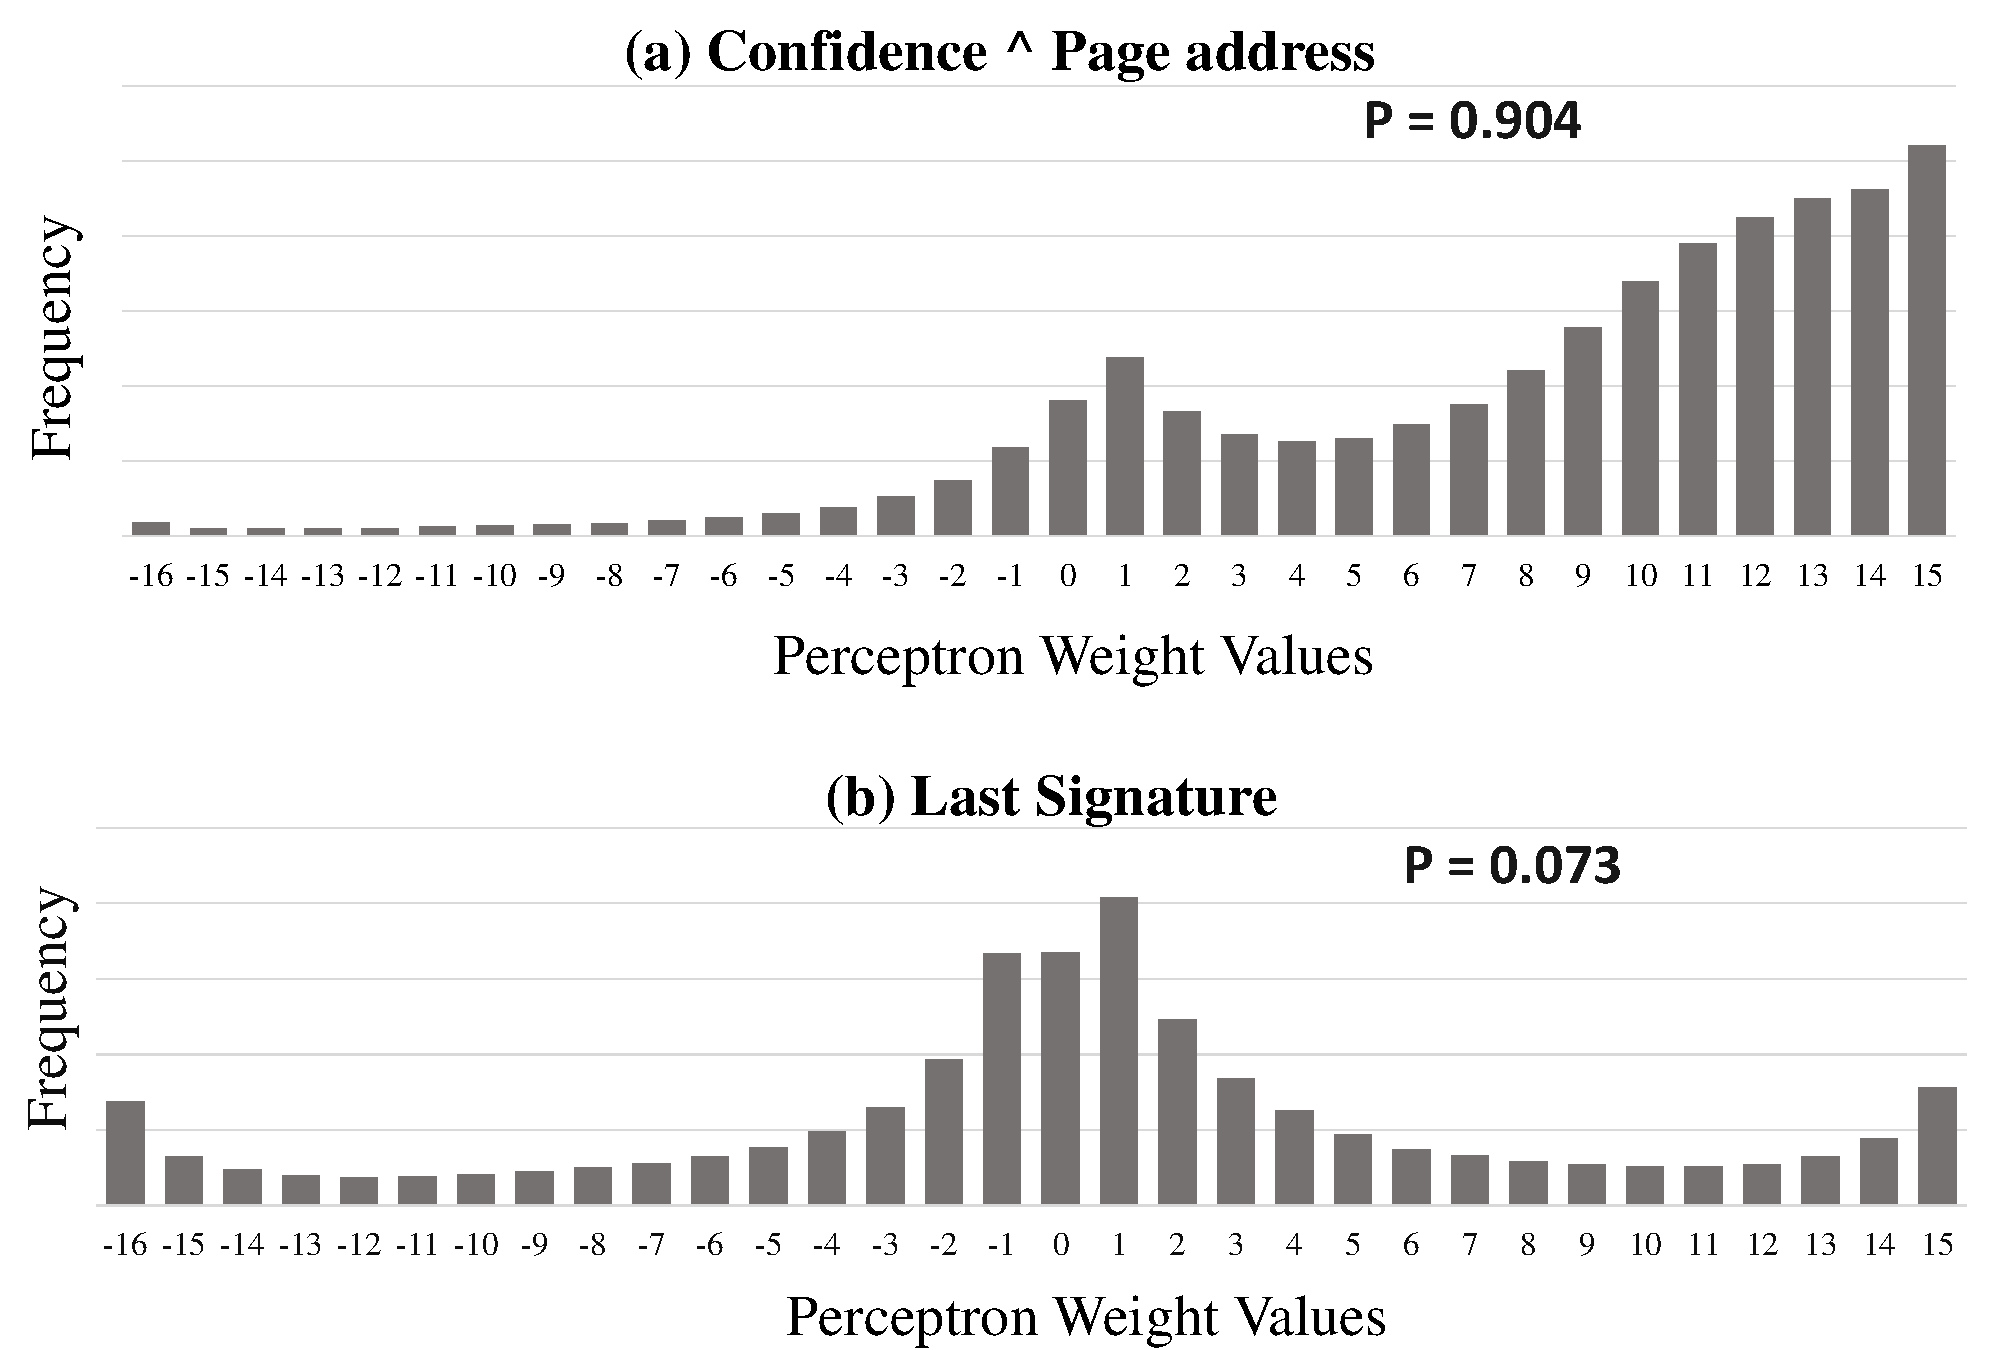
\includegraphics[width=\columnwidth]{Hist}
    \caption{Distribution of Trained Weights}
    \label{Fig:Hist}
  \end{center}
\end{figure}

\begin{figure}[h]
  \begin{center}
    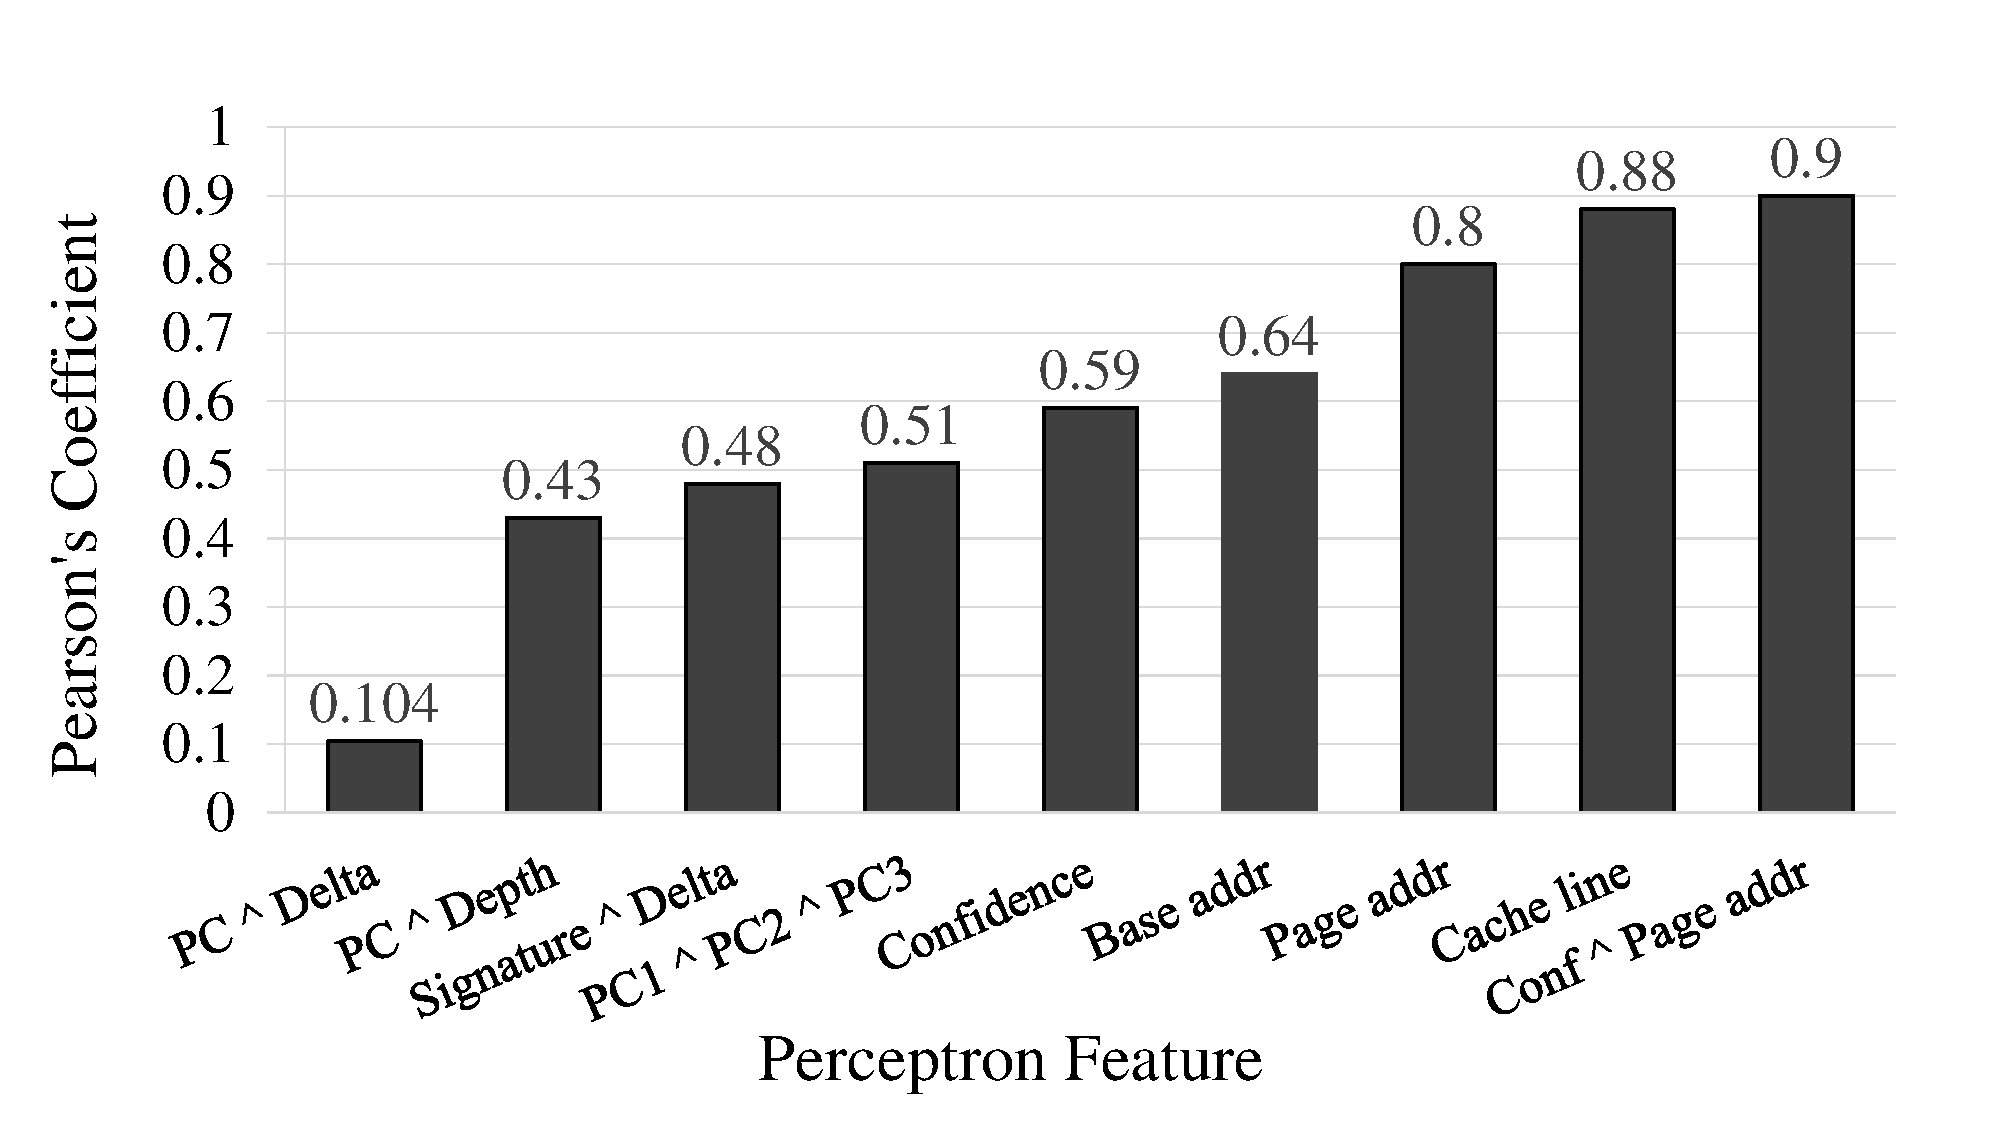
\includegraphics[width=\columnwidth]{Pvals}
    \caption{P-Values for all Features}
    \label{Fig:Pvals}
  \end{center}
\end{figure}


\begin{figure}[h]
  \begin{center}
    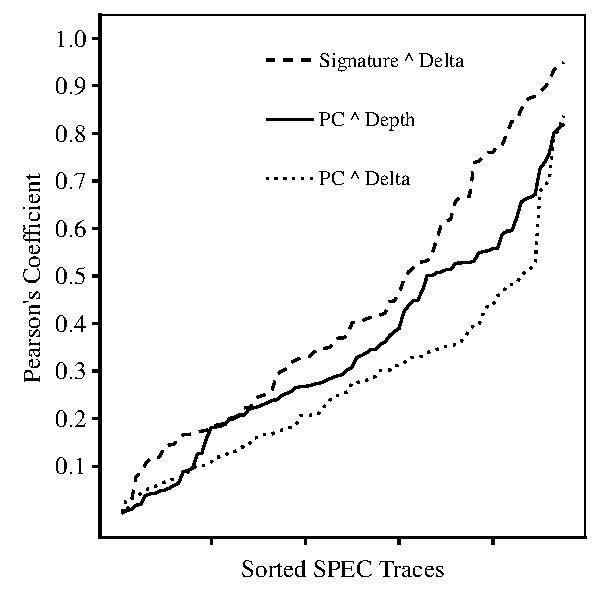
\includegraphics[width=\columnwidth]{Pvals_Trace}
    \caption{P-value Variation across Traces for selected Features}
    \label{Fig:Pvals_Trace}
  \end{center}
\end{figure}

We plot a histogram for each feature depicting weights distribution from -16
to +15 and generate the Pearson's correlation factor for that feature.
Pearson's factor is a numerical measure ranging from -1 to 1 of the degree of
linear correlation between two variables. The magnitude of Pearson's factor
gives the extent of correlation and the sign indicates whether it is a
positive correlation or a negative correlation. Values close to 0 suggest a
low correlation or at times, noisy data. A value of +1/-1 suggests a
perfectly linear positive / negative correlation respectively.

As a part of our perceptron feature selection methodology, we explored a wide 
variety of features to begin with. Features with a low 
Pearson's coefficient were rejected as they didn't provide much useful 
correlation. Figure~\ref{Fig:Hist} depicts the histogram distribution of 
trained weights for two features. The first feature, 
\textit{Confidence XOR Page address} has the highest observed P-value, 
hence was retained. On the other hand, the second feature, \textit{Last Signature}
did not provide any meaningful correlation and hence was rejected. 
This is visible from the bulk of its trained weights settling to near zero values.

Figure~\ref{Fig:Pvals} shows all the features which are finally used, 
arranged in the increasing order of their Pearson's factor. 
As can be seen 5 out of the 9 features provide a moderate to high 
correlation, with the magnitude of P-value > 0.6. The single most 
important feature, \textit{Confidence XOR Page address} helps provide
a correlation to prefetch outcome with a factor of 0.90. \\ \\
%
\textbf{Per Trace Correlation} \newline Another important way to look
at the perceptron features is to see how much their contribution
varies across the traces. Here we give special attention to features
with low P-values in. Figure~\ref{Fig:Pvals_Trace} shows the
variation of P-values for three features : \textit{PC XOR Delta},
\textit{Signature XOR Delta} and 
\textit{PC XOR Depth}; across all the SPEC CPU 2017 traces. 
For simplicity, the traces are arranged in an
increasing order of contribution made by the. 
It can be seen that even features with a low
overall correlation provide useful correlation (magnitude > 0.5) for
a significant number of traces. \\ \\
%
\textbf{Trimming Features Using Cross-correlation} \newline Beside
providing interesting insights into prefetching behavior, P-value can
also be used for feature selection and prefetcher tuning.

As we examined correlation of each feature with the final outcome, we also
studied correlation between the features. We used the above methodology to
eliminate features providing little information that has already been captured
in other features.

We initially came up a mix of 23 features. By studying
cross correlation of each of these features against others in a 23$\times$23
matrix, we identified pairs of features with correlation factor > 0.9 in
magnitude and eliminated redundant features, reducing the feature count to 9.
Thus, in the final implementation of PPF, no two features have a high
correlation between them. This way we can be sure that each feature makes a
contribution that cannot be captured using other features.

Secondly, studying the relative importance of each feature enabled us to vary
the number of entries dedicated for each feature. Features with higher
correlation, \textit{cache line} and \textit{page address} were given most
importance and allowed full 12-bits of indexing. Features like \textit{PC XOR
delta} and \textit{PC XOR depth} with a low overall P-value were allocated
fewer entries in the feature table.

%To conclude, in the above discussion we justify the features for
%perceptron from a statistical viewpoint.  We also show how this
%information can also be used for prefetcher tuning.  All this study
%was made possible only because we used on-line perceptron learning for
%prefetching and that enabled us to examine the weights in detail.

\begin{table}[ht]
    \centering
    \begin{tabular}{|c|c|c|}
    \hline
        \textbf{Field} &
        \textbf{Bits} &
        \textbf{Comment} \\
    \hline
         Valid 		& 1  & Indicates a valid entry in the table\\
         Tag 		& 6  & Identifier for the entry in the table\\
         \multirow{2}{1cm}{Useful} 	& 1  & To show if the given entry led to a\\
                    	&    & useful demand fetch\\
         Perc Decision 	& 1  & Prefetched vs Not-prefetched \\
    \hline
        PC 		& 12 & \\
        Address 	& 24 & \\
        Curr Signature 	& 10 & \multirow{2}{4.8cm}{Meta-data required for perceptron}\\
	PC$_i$ Hash	& 12 & \multirow{2}{1.1cm}{training}\\
        Delta 		& 7  & \\
        Confidence 	& 7  & \\
	Depth		& 4  & \\
    \hline
        \multicolumn{3}{|c|}{\textbf{Total 85 bits}}\\
    \hline
    \end{tabular}
    \caption{Meta-data Stored in Prefetch Table}
    \label{tab:PTable_metadata}
\end{table}


\subsection{Overhead for PPF}
\label{Method-Overheads}
In this section, we analyze the hardware overhead required to
implement PPF. The Prefetch Table was enhanced to accommodate
storing of meta-data for perceptron training. Table
\ref{tab:PTable_metadata} depicts the meta-data stored for each entry in
the Prefetch Table. Table \ref{tab:PPF_overhead} shows the total
storage overhead of PPF implementation. The hardware budget for
2nd Data Prefetching championship was 32 KB. Keeping that in mind 
the considerable speedup PPF obtained over the winner, the extra hardware
budget can be accounted for. The extra hardware also makes the
overall scheme more scalable than SPP. In the original SPP paper, it
was demonstrated that adding extra hardware brings little advantage in
terms of performance gain. The newly added perceptron tables can be
scaled to increase / decrease features depending on the permitted
budget.

\begin{table}[h]
\begin{adjustwidth}{-0.1cm}{}
    \centering
    \begin{tabular}{|c|c|c|c|}
    \hline
        \textbf{Structure} &
        \textbf{Entry} &
        \textbf{Components} &
        \textbf{Total} \\
    \hline
                                            &  \multirow{5}{0.5cm}{256}    & Valid (1 bit)  &             \\
                                             &      & Tag (16 bits)        &  \multirow{2}{0.9cm}{11008}           \\
                            Signature Table  &   & Last Offset (6 bits) &  \multirow{2}{0.5cm}{bits}  \\  
                                             &      & Signature (12 bits)  &             \\
                                             &      & LRU (6 bits)         &             \\
    \hline
                                    &  \multirow{3}{0.5cm}{512}    & $C_{sig}$ (4bits)      &\multirow{2}{0.9cm}{24576}               \\
                       Pattern Table         &   & $C_{delta}$ (4*4 bits) &  \multirow{2}{0.5cm}{bits}  \\
                                             &      & Delta (4*7 bits)       &               \\
    \hline
        \multirow{4}{1.5cm}{Perceptron\newline}     & 4096*4    & \multirow{4}{0.8cm}{5 bits}  & \multirow{3}{1.1cm}{113280}             \\
        \multirow{3}{1.2cm}{Weights}                & 2048*2    &           &  \multirow{3}{0.5cm}{bits}  \\
                                                    & 1024*2    &           &               \\
                                                    & 128*1     &           &              \\
    \hline
        Prefetch                & \multirow{2}{0.7cm}{1024}      & \multirow{2}{1cm}{85 bits}       & 87040 \\
        Table\footnotemark[1]   &           &               & bits\\
    \hline
        Reject                & \multirow{2}{0.7cm}{1024}      & \multirow{2}{1cm}{84 bits}    & 86016 \\
        Table\footnotemark[2] & & & bits\\
    \hline
        \multirow{4}{1.0cm}{Global\newline\newline}   & \multirow{4}{0.2cm}{8} & Signature (12 bits)  & \multirow{4}{1.1cm}{264 bits} \\
        \multirow{3}{1.1cm}{History\newline}        &                        & Confidence (8 bits)  &                               \\
        \multirow{2}{1.2cm}{Register}               &                        & Last Offset (6 bits) &                               \\
                                                    &                        & Delta (7 bits)       &                               \\
    \hline
        Accuracy        & 1     & C$_{total}$       & 10 bits   \\
        Counters        & 1     & C$_{useful}$      & 10 bits   \\
    \hline
        \multirow{3}{1.5cm}{Global PC\newline}      &       & $PC_1$ (12 bits)      &           \\
        \multirow{2}{1.5cm}{~Trackers}              & 3     & $PC_2$ (12 bits)      & 36 bits   \\
                                                    &       & $PC_3$ (12 bits)      &           \\
    \hline
        \multicolumn{4}{|c|}{\textbf{Total: 3,222,940 bits = 39.34 KB}}\\
    \hline
    \end{tabular}
    \caption{SPP-Perc Storage Overhead}
    \label{tab:PPF_overhead}
\end{adjustwidth}
\end{table}


\footnotetext[1]{Components of Prefetch Table can be found in Table \ref{tab:PTable_metadata}}
\footnotetext[2]{The Reject Table does not need to maintain the useful bit as that only applies for prefetches that ultimately made through}


In terms of computations, the perceptron mechanism only introduces an
extra adder tree. The hash perceptron mechanism makes sure than there
is no actual vector multiplication happening in the hardware.
Obtaining the perceptron sum requires addition of 9 5-bit numbers.
Using an adder tree of 4 5-bit adders, this can be done in
ceil($log_{2}9$) = 4 steps. Perceptron update only requires weight
update by +1 or -1. Thus, all the operations required for perceptron
inferencing or updating the states of the perceptrons can be
easily done in the time constraints of L2 Cache Accesses.

